% -----------------------------------------------------------------------------
% June 1, 2016
% This file contains a sample Bridges paper in LaTeX format.
% It has been prepared by Doug McKenna, using previous
% versions by Craig Kaplan, Reza Sarhangi, and others.
% It has been vetted using TeXShop 2.36 on Mac OS X (10.6).
% TeXShop is part of the TeX Live distribution, available
% at http://www.tug.org/texlive/
%
% -----------------------------------------------------------------------------

\documentclass[11pt]{article}
\usepackage{amsmath, amsthm, amssymb}    % May not all be necessary
\usepackage{bridges}                     % Custom bridges proceedings style
\usepackage{graphicx}                    % For including pictures
\usepackage{hyperref}                    % For formatting (clickable) URLs
\usepackage{subcaption}		     % Aaron added this one for certain figures

% -----------------------------------------------------------------------------

\title{Seeing and Hearing the Eigenvectors of a Fluid}
\author{ Aaron Demby-Jones, JoAnn Kuchera-Morin and Theodore Kim\\
Media Arts and Technology Program\\ University of California, Santa Barbara\\
{\tt aaron.demby.jones@mat.ucsb.edu, jkm@create.ucsb.edu, kim@mat.ucsb.edu}
}
% TK: MAT is a Program, not a Department. On my side, this is an MAT project, not a Pixar project.

% \date{[Draft as of \today]}	% For your own draft purposes
\date{}				% Suppress any date on submissions

% -----------------------------------------------------------------------------

\begin{document}

% -----------------------------------------------------------------------------
% Aaron's convenience commands
\newcommand{\UU}{\mathbf{U}}
\newcommand{\uu}{\mathbf{u}}
\newcommand{\vv}{\mathbf{v}}
\newcommand{\utilde}{\mathbf{q}}
\newcommand{\ff}{\mathbf{f}}
\newcommand{\qq}{\mathbf{q}}
\newcommand{\aaa}{\mathbf{a}}
\newcommand{\R}{\mathbb{R}}
% -----------------------------------------------------------------------------
% Ted's commands
\newcommand{\todo}[1]{$\spadesuit$ {\bf #1} $\spadesuit$}

\maketitle

% Prevent page number 1 from being printed on the first page.
\thispagestyle{empty}

\begin{abstract}
The intricate shapes and sounds that arise from the eigenvectors of vibrating Chladni plates are a well-known phenomenon. We explore a similar phenomenon by computing and visualizing the patterns formed by the empirical eigenvectors of a computational fluid dynamics simulation. The eigenvectors form complex, turbulent, spatial patterns. The eigenvalues form a spectrum that does not possess a unique sonic mapping, so we construct a sonification that allows us to listen to the trajectory of the fluid.
\end{abstract}

% Bridges papers are usually no more than 8 pages in length.  So
% there's really no need to have numbered sections, unless the
% author really needs to refer to sections within the paper's text.  So to suppress
% sequential section numbers, append an asterisk to the \section command, as in:

%%%%%%%%%%%%%%%%%%%%%%%%%%%%%%%%%%%%%%%%%%%
\section*{Introduction}

Chladni plates beautifully reveal the vibration modes, also known as the eigenvectors, of a rigid plate (Fig.~\ref{fig:chladni-drawn}). These eigenvectors can be computed analytically, as they correspond to very small deformations (i.e.~vibrations) on a very simple domain, and can be written in terms of the Laplacian operator $(\Delta)$ over a square domain. These visual representations can be extended to more complex scenarios, where the eigenvectors and their corresponding eigenvalues are instead computed numerically. In this work, we compute the eigenvectors of a dynamic computational fluid dynamics simulation, which involves large deformations instead of small vibrations, and the Navier-Stokes equations in lieu of a Laplacian. We then visualize the turbulent motion of the eigenvectors in this spectral representation, and construct a sonification of the resulting frequencies to produce a mapping between fluid trajectories and sound. The results are organic visual forms with a unique visual character, and sounds with \todo{say something nice about the sounds}.

\begin{figure*}
\centering
	\begin{subfigure}[h]{0.4\textwidth}
		\centering
		\includegraphics[width=\textwidth]{Figures/chladni_drawing.png}
		\caption{A table of hand-drawn Chladni figures. Source: Wikimedia Commons.}
		\label{fig:chladni-drawn}
	\end{subfigure}
	%
	 \hspace{3em}
	\begin{subfigure}[h]{0.4\textwidth}
		\centering
		\includegraphics[width=\textwidth]{Figures/chladni_plate.jpg}
		\caption{The physical experiment with a rectangular plate. Source: Wikimedia Commons.}
		\label{fig:chladni-plate}
	\end{subfigure}
\end{figure*}

\section*{Subspace fluids}
(/PLACEHOLDER)
While many subspace fluid simulation algorithms have been developed for computer graphics, they all use Galerkin projection. The basic strategy of this approach is to represent a large-dimensional velocity field in terms of a linear combination of a small number of carefully chosen basis vectors. To that end, a large-dimensional velocity field that contains $3N$ degrees of freedom over $N$ grid cells is projected into a smaller, $r$-dimensional velocity subspace $S \simeq \R^{r}$ using a static linear basis. We denote this change-of-basis matrix as $\UU \in \R^{3N \times r}$, where each column of $\UU$ is itself a velocity field. Specifically, we can project a vector $\uu \in \R^{3N}$ down to its reduced-order counterpart $\qq \in \R^r$ by computing the product $\UU^T \uu = \qq$. In a well-designed subspace simulation, the velocity fields spanned by the columns of $\UU$; i.e., the subspace $S$, will be sufficient to capture the space of fields that interest the user. This projection often occurs at the beginning of each timestep, as a force vector $\ff$ that contains important information such as user inputs, buoyancy, and vorticity confinement forces must be projected into the subspace.

Once this projection has been performed, the equations of motion can be integrated over this reduced number of variables very quickly. This can be done using exponential integration, Stable Fluids-like semi-Lagrangian advection coupled with Chorin projection, variational integration, or even simple explicit Euler integration. Once time integration has been performed, the change-of-basis must be reversed so that the results can be displayed. This is known as the ``velocity reconstruction'' stage. The most direct method is a {\em full} reconstruction where the $3N$-dimensional velocity field is reconstructed directly, i.e.~$\uu = \UU\qq$; and it is the approach we take in this paper.
(/endPLACEHOLDER)

In previous work, the subspace $S$ is discovered by first performing an appropriate training simulation at the full dimension and performing a singular value decomposition. Discarding the singular values less than a small threshold leaves us with $r$ singular values, with $r \ll 3N$, and their corresponding $r$ singular vectors, which are the basis vectors in the full space $\R^{3N}$ that generate $S$. In an analogy to the Chladni plate vibrations, these singular vectors correspond to the eigenfunctions, and the singular values correspond to the frequencies.


%\begin{figure*}
  %\begin{subfigure}[h]{0.62\textwidth}
    %\includegraphics[width=\textwidth]{Figures/principal_singular.eps}
%    \caption{Comparison of compression errors for plume.}
    %\label{fig:principal}
  %\end{subfigure}
  %
  % \begin{subfigure}[h]{0.62\textwidth}
    %\includegraphics[width=\textwidth]{Figures/min_singular.eps}
 %   \caption{Comparison of compression errors for sphere.}
    %\label{fig:min}
    %\end{subfigure}
     % \vspace{-3em}
 %\caption{Principal singular vector and minimal singular vector for the plume scene, respectively.}
%\end{figure*}
    
For each time step of the subspace re-simulation, when we perform the reconstruction phase, obtaining a full-space velocity field $\vv \in \R^{3N}$ from a reduced-order subspace vector $\qq \in \R^r$, we are simply taking a linear combination of the $r$ singular vectors using the corresponding coefficients given by the entries of $\qq$.
Hence, the subspace vectors $q$ can be intuitively thought of as instructions for how to mix together the corresponding singular vectors with the appropriate weightings. Indeed, we can even identify a path $\varphi \colon [0, 1] \rightarrow S$, sampled at $T$ timesteps $\varphi_1, \ldots, \varphi_T$, as determining the corresponding $T$ timesteps of the full-space re-simulation, after reconstruction.

%%%%%%%%%%%%%%%%%%%%%%%%%%%%%%%%%%%%%%%%%%%
\section*{Sonification}
We interpret the $r$ singular values $\sigma_1, \ldots, \sigma_r$ from the singular-value decomposition as characteristic frequencies. 

\begin{figure*}
	\begin{subfigure}[h]{0.5\textwidth}
		\includegraphics[width=\textwidth]{figures/singulars.eps}
		\caption{\textbf{Singular values: r = 50.} Note the logarithmic scale on the y-axis.}
		\label{fig:singulars}
	\end{subfigure}
	%
	\begin{subfigure}[h]{0.5\textwidth}
		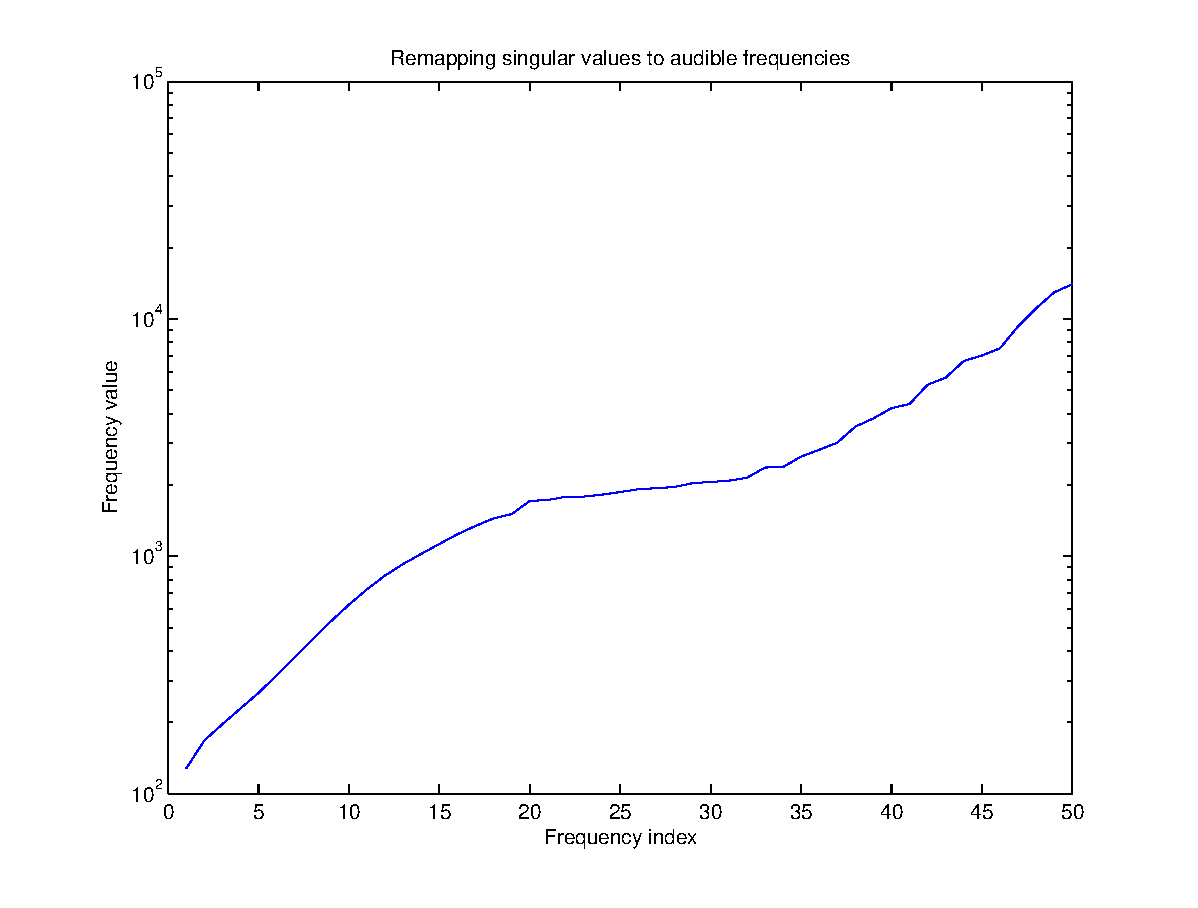
\includegraphics[width=\textwidth]{figures/remap_freqs.eps}
		\caption{\textbf{Remapped frequencies: f = 128 Hz, s = 6.} Note again the logarithmic scale on the y-axis.}
		\label{fig:freqs}
	\end{subfigure}
\end{figure*}

There are two immediate concerns about the raw data. Firstly, from Figure \ref{fig:singulars}, we see that the values range over approximately $12$ orders of magnitude, which is approximately $40$ octaves. However, the human audible dynamic range is generally considered to be from $20$ Hz to $20000$ Hz, which is only about $10$ octaves. Thus, we will have to rescale the octaves into an appropriate range. Secondly, starting from the principal singular value, the singular values are decreasing, whereas an audio spectrum increases from its fundamental frequency. Hence, we will have to invert the singular values. One way to proceed with a sensible mapping is to specify a desired fundamental frequency $f$ and an octave scaling $s$. Writing our audible frequencies as $f_1, \ldots, f_r$, we can define our mapping from singular values to audible frequencies as follows:

\begin{equation} 
\begin{aligned}
f_i &= f \cdot \left(\frac{\sigma_{i}^{-1}}{\sigma_{\textnormal{max}}^{-1}}\right)^{\frac{1}{s}} \\
&= f \cdot \left(\frac{\sigma_{\textnormal{max}}}{\sigma_i}\right)^{\frac{1}{s}}, \ i = 1, \ldots, r.
\end{aligned}
\end{equation}

The effect of this remapping can be seen in Figure \ref{fig:freqs}, where we have used a fundamental frequency $f = 128$ Hz and an octave scaling of $s = 6$. The spectrum now begins at the fundamental, $f = 128$ Hz, and ranges up to a maximum of approximately $14000$ Hz, an acceptable spread.

With an audible spectrum in hand, we now turn to the problem of choosing amplitudes for each individual frequency. These can be mapped from a corresponding subspace vector $\qq \in S$, as each of its $r$ components, $q_1, \ldots, q_r$ can be thought of as an amplitude for the $r$ corresponding frequencies $f_1, \ldots, f_r$. Care must be taken here too, as the overall sum of all the frequencies can exceed unity gain, and thus lead to clipping. Mathematically, this means that we require the $L^1$ norm of $\qq$, $\lvert\qq\rvert_1 = \sum_{i=1}^{r}\lvert q_i \rvert$, to be at most $1$. A typical subspace vector $\qq$ may also contain negative components. However, these can simply be thought of as encoding a positive amplitude and a reversal of phase. The phase reversal can be discarded, as its perceivable effect is typically undesirable clicking artifacts.

With these considerations in hand, we design a mapping from a subspace vector $\qq$ to an amplitude vector $\aaa$ of unit $L^1$ norm as follows:
\begin{equation}
\begin{aligned}
a_i &= \frac{\lvert q_i \rvert}{\lvert\qq\rvert_1}, \ i = 1, \ldots, r.
\end{aligned}
\end{equation}
Given a sequence $(\qq_j)$ of vectors that describe a sampled trajectory $\qq_1, \ldots, \qq_T$ through the subspace $S$, we can either normalize each one of the corresponding amplitude vectors on an individual basis, or we can determine the subspace vector of maximum $L^1$ norm, $\qq_{\textnormal{max}}$, and normalize each amplitude vector based on $\lvert\qq_{\textnormal{max}}\rvert_1$. The effect of the former is a relatively uniform volume level, while the effect of the latter is usually a significant audible decay from the first time step to the last, as in general, the first few $\qq$ vectors have a significantly higher $L^1$ norm than the remaining. Each approach thus has its musical merit, depending on the compositional situation.


\begin{figure*}
	\begin{subfigure}[h]{0.5\textwidth}
		\centering
		\includegraphics[width=\textwidth]{Figures/renders/plume0008.png}
			%\caption{A table of hand-drawn Chladni figures. Source: Wikimedia Commons.}
		%\label{fig:chladni-drawn}
	\end{subfigure}
	%
	% \hspace{3em}
	\begin{subfigure}[h]{0.5\textwidth}
		\centering
		\includegraphics[width=\textwidth]{Figures/renders/plume0009.png}
		%\caption{The physical experiment with a rectangular plate. Source: Wikimedia Commons.}
		%\label{fig:chladni-plate}
	\end{subfigure}
	\begin{subfigure}[h]{0.5\textwidth}
		\centering
		\includegraphics[width=\textwidth]{Figures/renders/plume0010.png}
		%\caption{The physical experiment with a rectangular plate. Source: Wikimedia Commons.}
		%\label{fig:chladni-plate}
	\end{subfigure}
	\begin{subfigure}[h]{0.5\textwidth}
		\centering
		\includegraphics[width=\textwidth]{Figures/renders/plume0011.png}
		%\caption{The physical experiment with a rectangular plate. Source: Wikimedia Commons.}
		%\label{fig:chladni-plate}
	\end{subfigure}
	\begin{subfigure}[h]{0.5\textwidth}
		\centering
		\includegraphics[width=\textwidth]{Figures/renders/plume0012.png}
		%\caption{The physical experiment with a rectangular plate. Source: Wikimedia Commons.}
		%\label{fig:chladni-plate}
	\end{subfigure}
	\begin{subfigure}[h]{0.5\textwidth}
		\centering
		\includegraphics[width=\textwidth]{Figures/renders/plume0013.png}
		%\caption{The physical experiment with a rectangular plate. Source: Wikimedia Commons.}
		%\label{fig:chladni-plate}
	\end{subfigure}
	\begin{subfigure}[h]{0.5\textwidth}
		\centering
		\includegraphics[width=\textwidth]{Figures/renders/plume0014.png}
		%\caption{The physical experiment with a rectangular plate. Source: Wikimedia Commons.}
		%\label{fig:chladni-plate}
	\end{subfigure}
	\begin{subfigure}[h]{0.5\textwidth}
		\centering
		\includegraphics[width=\textwidth]{Figures/renders/plume0015.png}
		%\caption{The physical experiment with a rectangular plate. Source: Wikimedia Commons.}
		%\label{fig:chladni-plate}
	\end{subfigure}
	
\end{figure*}

%%%%%%%%%%%%%%%%%%%%%%%%%%%%%%%%%%%%%%%%%%%
\section*{Synthesis}
With our mappings carried out, we can now produce sensible audible sound. The most basic technique to try is additive synthesis---namely, mixing together pure sine tones at the corresponding frequencies and amplitudes, creating an overall sound with a rich spectral content. With an instrument in hand that can produce the corresponding sound given a set of input amplitudes (SuperCollider's `DynKlang' unit generator is a suitable choice), a particular trajectory $\phi \colon [0, 1] \rightarrow S$ through the subspace, while retaining the same set of frequencies throughout time, determines a time-varying set of amplitudes, allowing the subspace evolution to dictate the time evolution of the sound. The overall effect is a subtle change in timbre, as the amplitudes of the various overtones fluctuate.

Subtractive synthesis is also an interesting option. We start with a spectrally rich input sound, such as an impulse or broadband noise. We then create a filter bank of resonances at the appropriate set of frequencies, weighted in turn by the appropriate set of amplitudes. (The SuperCollider unit generator `DynKlank' is the point of departure on an implementation level.) Some extra parameters must be addressed, as each resonant mode also is given a ring time for the mode to decay by $60$ dB. The nature of the input sound also strongly influences the resulting timbre---broadband noise creates a more atmospheric effect, while impulses can create driving rhythmic textures. 

%%%%%%%%%%%%%%%%%%%%%%%%%%%%%%%%%%%%%%%%%%%
\section*{Time evolution}
Static sound, while interesting as a new timbre for a few seconds, eventually grows stale. Thus, we would like to capture the time evolution of the subspace trajectory as a dynamic sonic event. This can be achieved by cycling through the the sequence of amplitude vectors $\aaa_1, \ldots, \aaa_T$ corresponding to the subspace trajectory $\qq_1, \ldots, \qq_T$. Indeed, different trajectories through the subspace generated different sequences of amplitude vectors. The unfolding of these trajectories over time occurs on a micro-scale musically, but the choice of different possible abstract trajectories, and the shifting from one trajectory to another, is expressed on more of a meso- or even macro-level scale.

Experimentally, we have explored several different categories of subspace trajectories. The simplest is the original subspace re-simulation trajectory, which is faithful to the original simulation. Another possibility is the `frequency response' trajectory, which is the result of setting the first subspace vector $\qq_1 = \mathbf{1}$, the vector of all $1s$, and allowing the simulation to unfold from there. Both of these possibilities retain the original physics-based dynamics to update each timestep. It is also possible, however, to abandon the physics and simply choose a trajectory by other means. For example, starting from the same initial vector $\qq_1$ as in the original re-simulation, we can determine a trajectory simply by walking in a random direction at each time step, or walking along the surface of some abstract manifold $M \subset S$, such as a sphere. These lead both to unique visual and aural results. 

Since the the set of frequencies itself remains static over time, and only the amplitudes are changing, musically, it will also make sense to explore dynamically changing the pitch $f$ which was specified as the original fundamental frequency. This can be achieved simply by multiplying the entire spectrum by an interval, which will create a new fundamental without affecting the ratios between the partials. Alternatively, we could consider the original spectrum as a musical scale with which to compose melodies if we desire to compose more at the note scale.

%%%%%%%%%%%%%%%%%%%%%%%%%%%%%%%%%%%%%%%%%%%



%%%%%%%%%%%%%%%%%%%%%%%%%%%%%%%%%%%%%%%%%%%

% If you are only going to use a BibTeX database, from which all your cites will be
% taken and formatted consistently, use the following.

\bibliographystyle{plain}
\fontsize{10}{12}
\bibliography{mybib}

\end{document}